\documentclass[11pt,a4paper]{article}

% These are extra packages that you might need for writing the equations:
\usepackage{amsmath}
\usepackage{amsfonts}
\usepackage{amssymb}

% You need the following package in order to include figures in your report:
\usepackage{graphicx}

% With this package you can set the size of the margins manually:
\usepackage[left=2cm,right=2cm,top=2cm,bottom=2cm]{geometry}


\begin{document}

% Enter the exercise number, your name and date here:
\noindent\parbox{\linewidth}{
 \parbox{.25\linewidth}{ \large HPCSE I, Exercise xx }\hfill
 \parbox{.5\linewidth}{\begin{center} \large Beat Hubmann \end{center}}\hfill
 \parbox{.2\linewidth}{\begin{flushright} \large Sep 30, 2018 \end{flushright}}
}
\noindent\rule{\linewidth}{2pt}


\section{Introduction}

Briefly introduce the problem here. Describe what you have to do and what the goal is. Make sure to cite any references that you might use \cite{knuth}.

\section{Algorithm Description}

Briefly and accurately describe the algorithm that you use to solve the problem. Avoid unnecessary technical details. It is not necessary to include the code in the report. When necessary, to make a point or explain with greater clarity, you can include a code snippet. The source code should be included in a separate file and it is absolutely necessary that you \textbf{make sure that your source code is properly annotated, commented and indented}. 

\section{Results}

\subsection{Task x}
This is an example equation:
\begin{equation}
y = e^{-0.01x},
\end{equation}
which is plotted in figure \ref{fig:figure1} below.

\begin{figure}[ht]
\begin{center}
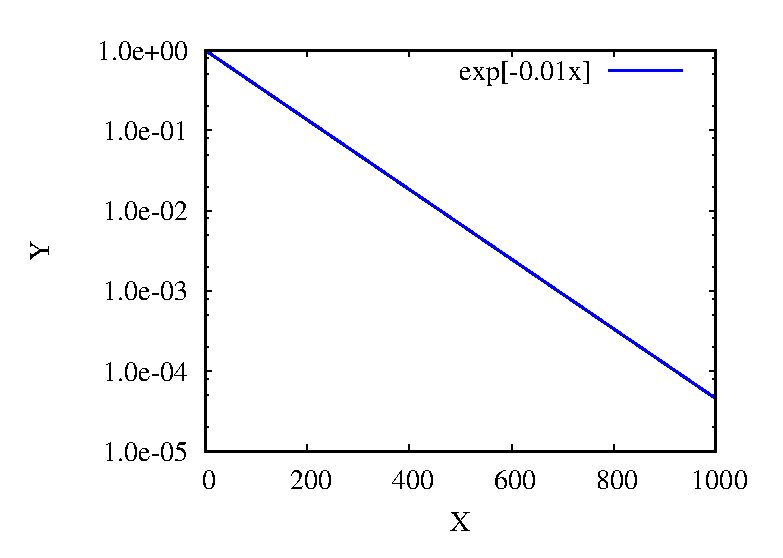
\includegraphics[scale=0.9]{figure.eps} 
\end{center}
\caption{Always \textbf{label your figures}! Make sure that you always \textbf{include a figure caption} where you state all the parameters used during the simulation for which the results in the figure were obtained. \textbf{Always label the axes!} If possible, state briefly what you can learn from the results, what do they tell us. When appropriate or necessary use a semi-log or a log-log scale! Make sure that the figure is nice and big as shown here.}
\label{fig:figure1}
\end{figure}


\subsection{Task y}
\subsection{Task z}

\section{Discussion}
Discuss your results and any problems that you might have encountered.

\begin{thebibliography}{99}

\bibitem{knuth}
  Knuth, Ervin D.,
  \emph{The art of computer programming}, 
  Addison Wesley, Massachusetts,
  3rd edition,
  1997.

\end{thebibliography}

\end{document}